\usetikzlibrary{positioning,shapes,arrows}

\newcommand{\bayesTicks}{
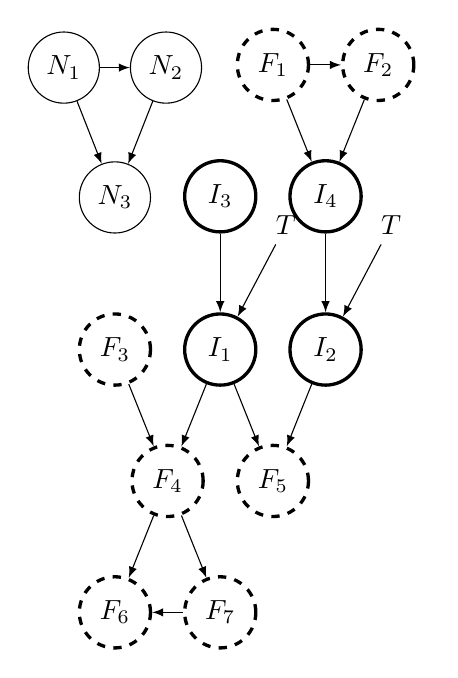
\begin{tikzpicture}[
  node distance=1cm and 0cm,
  mynode/.style={draw,ellipse,text width=2cm,align=center},
  Tnode/.style={text width=0.75cm,align=center},
  Inode/.style={draw,very thick,circle,text width=0.5cm,align=center},
  Fnode/.style={draw,very thick,dashed,circle,text width=0.5cm,align=center},
  Nnode/.style={draw,circle,text width=0.5cm,align=center}
]
% \node[mynode] (sp) {Sprinkler};
% \node[mynode,below right=of sp] (gw) {Grass wet};
% \node[mynode,above right=of gw] (ra) {Rain};
% \path (ra) edge[-latex] (sp)
% (sp) edge[-latex] (gw) 
% (gw) edge[latex-] (ra);


\node[Fnode                   ] (N01) {$F_1$}; 
\node[Inode,below right=of N01] (N04) {$I_4$}; 
\node[Fnode,above right=of N04] (N02) {$F_2$}; 
\node[Inode,below      =of N04] (N08) {$I_2$};
\node[Fnode,below left =of N08] (N10) {$F_5$}; 
\node[Inode,above left =of N10] (N07) {$I_1$}; 
\node[Inode,above      =of N07] (N03) {$I_3$}; 
\node[Tnode,above right=of N07] (N05) {$T$}; 
\node[Tnode,above right=of N08] (N06) {$T$}; 
\node[Fnode,below left =of N07] (N09) {$F_4$};  
\node[Fnode,below left =of N09] (N13) {$F_6$}; 
\node[Fnode,below right=of N09] (N14) {$F_7$}; 
\node[Fnode,above left =of N09] (N16) {$F_3$};

\node[Nnode,above      =of N16] (N15) {$N_3$}; 
\node[Nnode,above left =of N15] (N11) {$N_1$}; 
\node[Nnode,above right=of N15] (N12) {$N_2$};

\path (N01) edge[-latex] (N04);
\path (N02) edge[-latex] (N04);
\path (N03) edge[-latex] (N07);
\path (N04) edge[-latex] (N08);
\path (N05) edge[-latex] (N07);
\path (N06) edge[-latex] (N08);
\path (N07) edge[-latex] (N09);
\path (N07) edge[-latex] (N10);
\path (N08) edge[-latex] (N10);
\path (N09) edge[-latex] (N13);
\path (N09) edge[-latex] (N14);
\path (N11) edge[-latex] (N15);
\path (N12) edge[-latex] (N15);
\path (N16) edge[-latex] (N09);

\path (N11) edge[-latex] (N12);
\path (N14) edge[-latex] (N13);
\path (N01) edge[-latex] (N02);

\end{tikzpicture}
}